%%%%%%%%%%%%%%%%%%%%%%%%%%%%%%%%%%%%%%%%%
% Beamer Presentation
% LaTeX Template
% Version 1.0 (10/11/12)
%
% This template has been downloaded from:
% http://www.LaTeXTemplates.com
%
% License:
% CC BY-NC-SA 3.0 (http://creativecommons.org/licenses/by-nc-sa/3.0/)
%
%%%%%%%%%%%%%%%%%%%%%%%%%%%%%%%%%%%%%%%%%

%----------------------------------------------------------------------------------------
%	PACKAGES AND THEMES
%----------------------------------------------------------------------------------------

\documentclass[handout]{beamer}

\mode<presentation> {

% The Beamer class comes with a number of default slide themes
% which change the colors and layouts of slides. Below this is a list
% of all the themes, uncomment each in turn to see what they look like.

%\usetheme{default}
%\usetheme{AnnArbor}
%\usetheme{Antibes}
%\usetheme{Bergen}
%\usetheme{Berkeley}
%\usetheme{Berlin}
%\usetheme{Boadilla}
%\usetheme{CambridgeUS}
%\usetheme{Copenhagen}
%\usetheme{Darmstadt}
%\usetheme{Dresden}
%\usetheme{Frankfurt}
%\usetheme{Goettingen}
%\usetheme{Hannover}
%\usetheme{Ilmenau}
%\usetheme{JuanLesPins}
%\usetheme{Luebeck}
\usetheme{Madrid}
%\usetheme{Malmoe}
%\usetheme{Marburg}
%\usetheme{Montpellier}
%\usetheme{PaloAlto}
%\usetheme{Pittsburgh}
%\usetheme{Rochester}
%\usetheme{Singapore}
%\usetheme{Szeged}
%\usetheme{Warsaw}

% As well as themes, the Beamer class has a number of color themes
% for any slide theme. Uncomment each of these in turn to see how it
% changes the colors of your current slide theme.

%\usecolortheme{albatross}
%\usecolortheme{beaver}
%\usecolortheme{beetle}
%\usecolortheme{crane}
%\usecolortheme{dolphin}
%\usecolortheme{dove}
%\usecolortheme{fly}
%\usecolortheme{lily}
%\usecolortheme{orchid}
%\usecolortheme{rose}
%\usecolortheme{seagull}
%\usecolortheme{seahorse}
%\usecolortheme{whale}
%\usecolortheme{wolverine}

%\setbeamertemplate{footline} % To remove the footer line in all slides uncomment this line
%\setbeamertemplate{footline}[page number] % To replace the footer line in all slides with a simple slide count uncomment this line

%\setbeamertemplate{navigation symbols}{} % To remove the navigation symbols from the bottom of all slides uncomment this line
}

\usepackage{graphicx} % Allows including images
\usepackage{booktabs} % Allows the use of \toprule, \midrule and \bottomrule in tables
\usepackage{cool}
\usepackage{tikz}
\usepackage{amsmath}
\usepackage{xcolor}
\usepackage{hyperref}
\usepackage{bm}

\DeclareMathOperator*{\argmax}{argmax}
\DeclareMathOperator*{\argmin}{argmin}
\usetikzlibrary{positioning}

%----------------------------------------------------------------------------------------
%	TITLE PAGE
%----------------------------------------------------------------------------------------

\title[RL for Finance]{Reinforcement Learning and it's Applications in Finance\\ (A Thalesians Talk)} % The short title appears at the bottom of every slide, the full title is only on the title page

\author{Ashwin Rao} % Your name
\institute[Stanford] % Your institution as it will appear on the bottom of every slide, may be shorthand to save space
{Stanford University
 % Your institution for the title page
}

\date{July 14, 2021} % Date, can be changed to a custom date

\begin{document}
\begin{frame}
\titlepage % Print the title page as the first slide
\end{frame}

% \begin{frame}
% \frametitle{Overview} % Table of contents slide, comment this block out to remove it
% \tableofcontents % Throughout your presentation, if you choose to use \section{} and \subsection{} commands, these will automatically be printed on this slide as an overview of your presentation
% \end{frame}

\begin{frame}
\frametitle{About Me}
\pause
\begin{itemize}[<+->]
\item VP of AI at \href{https://www.target.com/}{\underline{\textcolor{blue}{Target Corporation}}} ($\sim$ \$100B US Retail Company)
\item Adjunct Professor, \href{https://icme.stanford.edu/}{\underline{\textcolor{blue}{Applied Math (ICME)}}}, Stanford University
\item Past: MD at Morgan Stanley, Trading Strategist at Goldman Sachs
\item Wall Street career mostly in Rates and Mortgage Derivatives
\item Educational background: Algorithms Theory and Abstract Algebra
\item I direct Stanford's \href{https://mcf.stanford.edu/}{\underline{\textcolor{blue}{Mathematical \& Computational Finance program}}}
\item Research \& Teaching in: {\em RL and it's applications in Finance \& Retail}
\item In-progress book:  \href{http://stanford.edu/~ashlearn/RLForFinanceBook/book.pdf}{\underline{\textcolor{blue}{Foundations of RL with Applications in Finance}}}
\item Book blends Theory, Modeling, Algorithms, Python, Trading problems
\item Emphasis on broader principles in Applied Math \& Software Design
\item I spend a lot of time writing  \href{https://github.com/TikhonJelvis/RL-book}{\underline{\textcolor{blue}{code associated with the book}}}
\end{itemize}
\end{frame}


\begin{frame}
\frametitle{AI for Dynamic Decisioning under Uncertainty}
\pause
\begin{itemize}[<+->]
\item Let's browse some terms used to characterize this branch of AI
\item {\em Stochastic}: Uncertainty in key quantities, evolving over time
\item {\em Optimization}: A well-defined metric to be maximized (``The Goal'')
\item {\em Dynamic}:  Decisions need to be a function of the changing situations
\item {\em Control}: Overpower uncertainty by persistent steering towards goal
\item Jargon overload due to confluence of Control Theory, OR and AI
\item For language clarity, let's just refer to this area as {\em Stochastic Control}
\item The core framework is called {\em Markov Decision Processes} (MDP)
\item {\em Reinforcement Learning} is a class of algorithms to solve MDPs
\end{itemize}
\end{frame}



\begin{frame}
\frametitle{The MDP Framework}
\includegraphics[width=12cm, height=7cm]{MDP.png}
\end{frame}

\begin{frame}
\frametitle{Components of the MDP Framework}
\pause
\begin{itemize}[<+->]
\item The {\em Agent} and the {\em Environment} interact in a time-sequenced loop
\item {\em Agent} responds to [{\em State}, {\em Reward}] by taking an {\em Action}
\item {\em Environment} responds by producing next step's (random) {\em State}
\item {\em Environment} also produces a (random) scalar denoted as {\em Reward}
\item Each {\em State} is assumed to have the {\em Markov Property}, meaning:
\begin{itemize}
\item Next {\em State/Reward} depends only on Current {\em State} (for a given {\em Action})
\item Current {\em State} captures all relevant information from {\em History}
\item Current {\em State} is a sufficient statistic of the future (for a given {\em Action})
\end{itemize} 
\item Goal of {\em Agent} is to maximize {\em Expected Sum} of all future {\em Reward}s
\item By controlling the ({\em Policy} : {\em State} $\rightarrow$ {\em Action}) function
\item This is a dynamic (time-sequenced control) system under uncertainty
\end{itemize}
\end{frame}

\begin{frame}
\frametitle{Formal MDP Framework}
The following notation is for discrete time steps. Continuous-time formulation is analogous (often involving
\href{https://github.com/coverdrive/technical-documents/blob/master/finance/cme241/StochasticCalculusFoundations.pdf}{\underline{\textcolor{blue}{Stochastic Calculus}}})
\pause
\begin{itemize}[<+->]
\item Time steps denoted as $t = 1, 2, 3, \ldots$
\item Markov States $S_t \in \mathcal{S}$ where $\mathcal{S}$ is the State Space
\item Actions $A_t \in \mathcal{A}$ where $\mathcal{A}$ is the Action Space
\item Rewards $R_t \in \mathbb{R}$ denoting numerical feedback\
\item Transitions $p(r,s'|s,a) = \mathbb{P}[(R_{t+1}=r,S_{t+1}=s')|S_t=s,A_t=a]$
\item $\gamma \in [0,1]$ is the Discount Factor for Reward when defining {\em Return}
\item Return $G_t = R_{t+1} + \gamma \cdot R_{t+2} + \gamma^2 \cdot R_{t+3} + \ldots$
\item Policy $\pi(a|s)$ is probability that Agent takes action $a$ in states $s$
\item The goal is find a policy that maximizes  $\mathbb{E}[G_t|S_t = s]$ for all $s \in \mathcal{S}$
\end{itemize}
\end{frame}

\begin{frame}
\frametitle{How a baby learns to walk}
\includegraphics[width=13cm, height=8cm]{BabyMDP.jpg}
\end{frame}

\begin{frame}
\frametitle{Many real-world problems fit this MDP framework}
\pause
\begin{itemize}[<+->]
\item Self-driving vehicle (speed/steering to optimize safety/time)
\item Game of Chess (Boolean {\em Reward} at end of game)
\item Complex Logistical Operations (eg: movements in a Warehouse)
\item Make a humanoid robot walk/run on difficult terrains
\item Manage an investment portfolio
\item Control a power station
\item Optimal decisions during a football game
\item Strategy to win an election (high-complexity MDP)
\end{itemize}
\end{frame}

\begin{frame}
\frametitle{Self-Driving Vehicle}
\includegraphics[width=13cm, height=8cm]{CarMDP.jpg}
\end{frame}

\begin{frame}
\frametitle{Why are these problems hard?}
\pause
\begin{itemize}[<+->]
\item {\em State} space can be large or complex (involving many variables)
\item Sometimes, {\em Action} space is also large or complex
\item No direct feedback on ``correct'' {\em Actions} (only feedback is {\em Reward})
\item Time-sequenced complexity ({\em Actions} influence future {\em States/Actions})
\item {\em Action}s can have delayed consequences (late {\em Reward}s)
\item {\em Agent} often doesn't know the {\em Model} of the {\em Environment}
\item ``Model'' refers to probabilities of state-transitions and rewards
\item So, {\em Agent} has to learn the {\em Model} AND solve for the Optimal {\em Policy}
\item {\em Agent} {\em Action}s need to tradeoff between ``explore'' and ``exploit''
\end{itemize}
\end{frame}

\begin{frame}
\frametitle{Value Function and Bellman Equations}
\pause
\begin{itemize}
\item Value function (under policy $\pi$) $V_{\pi}(s) = \mathbb{E}[G_t|S_t = s]$ for all $s \in \mathcal{S}$
\pause
$$V_{\pi}(s) = \sum_{a} \pi(a|s) \sum_{r,s'} p(r,s'|s,a) \cdot (r + \gamma V_{\pi}(s')) \mbox{ for all } s \in \mathcal{S}$$
\pause
\item Optimal Value Function $V_{*}(s) = \max_{\pi} V_{\pi}(s) \mbox{ for all } s \in \mathcal{S}$
\pause
$$V_{*}(s) = \max_{a} \sum_{r,s'} p(r,s'|s,a) \cdot (r + \gamma V_{*}(s')) \mbox{ for all } s \in \mathcal{S}$$
\pause
\item {\em There exists an Optimal Policy} $\pi_{*}$ achieving $V_{*}(s)$ for all $s \in \mathcal{S}$
\pause
\item Determining $V_{\pi}(s)$ known as {\em Prediction}, and $V_{*}(s)$ known as {\em Control}
\pause
\item The above recursive equations are called {\em Bellman equations}
\pause
\item In continuous time, refered to as {\em Hamilton-Jacobi-Bellman (HJB)}
\pause
\item The algorithms based on Bellman equations are broadly classified as:
\begin{itemize}
\item Dynamic Programming
\item Reinforcement Learning
\end{itemize}

\end{itemize}
\end{frame}


\begin{frame}
\frametitle{Dynamic Programming}
\pause
\begin{itemize}[<+->]
\item When Probabilities Model is known $\Rightarrow$ {\em Dynamic Programming} (DP)
\item DP Algorithms take advantage of knowledge of probabilities
\item So, DP Algorithms do not require interaction with the environment
\item In the Language of AI, DP is a type of {\em Planning Algorithm}
\item DP algorithms are iterative algorithms based on Fixed-Point Theorem
\item Finding a {\em Fixed Point} of Operator based on Bellman Equation
\item Why is DP not effective in practice?
\pause
\begin{itemize}[<+->]
\item Curse of Dimensionality
\item Curse of Modeling
\end{itemize}
\item Curse of Dimensionality can be partially cured with Approximate DP
\item To resolve both curses effectively, we need RL
\end{itemize}
\end{frame}

\begin{frame}
\frametitle{Reinforcement Learning}
\pause
\begin{itemize}[<+->]
\item Typically in real-world, we don't have access to a Probabilities Model
\item All we have is access to an environment serving individual transitions
\item Even if MDP model is available, model updates can be challenging
\item Often real-world models end up being too large or too complex
\item Sometimes estimating a {\em sampling model} is much more feasible
\item So RL interacts with either {\em actual} or {\em simulated} environment
\item Either way, we receive {\em individual transitions} to next state and reward
\item RL is a ``trial-and-error'' approach linking {\em Actions} to {\em Returns}
\item Try different actions \& learn what works, what doesn't
\item This is hard because actions have overlapping reward sequences
\item Also, sometimes Actions result in {\em delayed Rewards}
\end{itemize}
\end{frame}

\begin{frame}
\frametitle{RL: Learning Value Function Approximation from Samples}
\pause
\begin{itemize}[<+->]
\item RL incrementally learns the Value Function from transitions data
\item Appropriate Approximation of Value Function is key to success
\item Deep Neural Networks are typically used for function approximation
\item Big Picture: Sampling and Function Approximation come together
\item RL algorithms are clever about balancing  ``explore'' versus ``exploit''
\item Most RL Algorithms are founded on the Bellman Equations
\item {\bf Promise of modern A.I. is based on success of RL algorithms}
\item Potential for automated decision-making in many industries
\item In 10-20 years: Bots that act or behave more optimal than humans
\item RL already solves various low-complexity real-world problems
\item RL might soon be the most-desired skill in the technical job-market
\item Possibilities in Finance are endless (we cover 5 important problems)
\item Studying RL is a lot of fun! (interesting in theory as well as coding)
\end{itemize}
\end{frame}

\begin{frame}
\frametitle{Many Faces of Reinforcement Learning}
\includegraphics[width=9cm, height=8cm]{many_faces_of_RL.PNG}
\end{frame}

\begin{frame}
\frametitle{Vague (but in-vogue) Classification of Machine Learning}
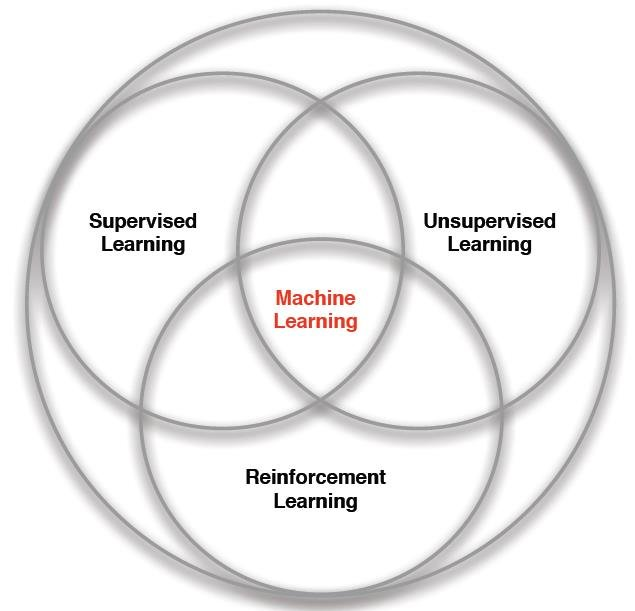
\includegraphics[width=9cm, height=8cm]{MLBranches.PNG}
\end{frame}

\begin{frame}
\frametitle{P1: Dynamic Asset-Allocation and Consumption}
\pause
\begin{itemize}[<+->]
\item The broad topic is Investment Management
\item Applies to Corporations as well as Individuals
\item The two considerations are:
\pause
\begin{itemize}[<+->]
\item How to allocate money across assets in one's investment portfolio
\item How much to consume for one's needs/operations/pleasures
\end{itemize}
\item We consider the dynamic version of these dual considerations
\item Asset-Allocation and Consumption decisions at each time step
\item Asset-Allocation decisions typically deal with Risk-Reward tradeoffs
\item Consumption decisions are about spending now or later
\item Objective: Horizon-Aggregated Expected \href{https://github.com/coverdrive/technical-documents/blob/master/finance/cme241/Tour-UtilityTheory.pdf}{\underline{\textcolor{blue}{Utility of Consumption}}}
\end{itemize}
\end{frame}

\begin{frame}
\frametitle{P1: Consider the simple example of Personal Finance}
\pause
\begin{itemize}[<+->]
\item Broadly speaking, Personal Finance involves the following aspects:
\pause
\begin{itemize}[<+->]
\item Receiving Money: Salary, Bonus, Rental income, Asset Liquidation etc.
\item Consuming Money: Food, Clothes, Rent/Mortgage, Car, Vacations etc.
\item Investing Money: Savings account, Stocks, Real-estate, Gold etc.
\end{itemize}
\item Goal: Maximize lifetime-aggregated Expected Utility of Consumption
\item This can be modeled as a Markov Decision Process
\item {\em State:} Age, Asset Holdings, Asset Valuation, Career situation etc.
\item {\em Action:} Changes in Asset Holdings, Optional Consumption
\item {\em Reward:} Utility of Consumption of Money
\item {\em Model:} Career uncertainties, Asset market uncertainties
\end{itemize}
\end{frame}

\begin{frame}
\frametitle{P1: Merton's Frictionless Continuous-Time Formulation}
\pause
\begin{itemize}[<+->]
\item Assume: Current wealth is $W_0 > 0$, and you'll live for $T$ more years
\item You can invest in (allocate to) $n$ risky assets and a riskless asset
\item Each risky asset has known normal distribution of returns
\item Allowed to long or short any fractional quantities of assets
\item Trading in continuous time $0 \leq t < T$, with no transaction costs
\item You can consume any fractional amount of wealth at any time
\item Dynamic Decision: Optimal Allocation and Consumption at each time
\item To maximize lifetime-aggregated Expected Utility of Consumption
\item Consumption Utility assumed to have Constant Relative Risk-Aversion
\end{itemize}
\end{frame}

\begin{frame}
\frametitle{P1: Problem Notation}
For simplicity, consider the case of 1 risky asset
\pause
\begin{itemize}[<+->]
\item Riskless asset: $dR_t = r \cdot R_t \cdot dt$
\item Risky asset: $dS_t = \mu \cdot S_t \cdot dt + \sigma \cdot S_t \cdot dz_t$ (i.e. Geometric Brownian)
\item $\mu > r > 0, \sigma > 0$ (for $n$ assets, we work with a covariance matrix)
\item Wealth at time $t$ is denoted by $W_t > 0$
\item Fraction of wealth allocated to risky asset denoted by $\pi(t, W_t)$
\item Fraction of wealth in riskless asset will then be $1 - \pi(t, W_t)$
\item Wealth consumption per unit time denoted by $c(t, W_t) \geq 0$
\item Utility of Consumption function $U(x) = \frac {x^{1-\gamma}} {1 - \gamma}$ for $0 < \gamma \neq 1$
\item $\gamma =$ (Constant) Relative Risk-Aversion $\frac {-x \cdot U''(x)} {U'(x)}$
\end{itemize}
\end{frame}

\begin{frame}
\frametitle{P1: Formal Problem Statement}
\pause
\begin{itemize}[<+->]
\item Write $\pi_t, c_t$ instead of $\pi(t, W_t), c(t, W_t)$ to lighten notation
\item Balance constraint implies the following process for Wealth $W_t$
$$dW_t = ((\pi_t \cdot (\mu - r) + r) \cdot W_t - c_t) \cdot dt + \pi_t \cdot \sigma \cdot W_t \cdot dz_t$$
\item At any time $t$, determine optimal $[\pi(t,W_t), c(t, W_t)]$ to maximize:
$$\mathbb{E}[\int_t^T \frac {e^{-\rho (s-t)} \cdot c_s^{1-\gamma}} {1-\gamma} \cdot ds + \frac {e^{-\rho (T-t)} \cdot B \cdot W_T^{1-\gamma}} {1-\gamma} \mid W_t]$$
where $\rho \geq 0$ is the utility discount rate, $B$ is the bequest
\item We can solve this problem for arbitrary bequest but Merton considers $B = \epsilon^{\gamma}$
where $0 < \epsilon \ll 1$, meaning ``zero" bequest
\end{itemize}
\end{frame}

\begin{frame}
\frametitle{P1: Continuous-Time Stochastic Control}
\begin{itemize}[<+->]
\item Think of this as a continuous-time Stochastic Control problem
\item The {\em State} at time $t$ is $(t, W_t)$
\item The {\em Action} at time $t$ is $[\pi_t, c_t]$
\item The {\em Reward} per unit time at time $t$ is $U(c_t) = \frac {c_t^{1 - \gamma}} {1 - \gamma}$ 
\item The {\em Return} at time $t$ is the accumulated discounted {\em Reward}:
$$\int_t^T e^{-\rho(s-t)} \cdot \frac {c_s^{1-\gamma}} {1-\gamma} \cdot ds$$
\item Find {\em Policy} $: (t, W_t) \rightarrow [\pi_t, c_t]$ that maximizes the {\em Expected Return}
\item Note: $c_t \geq 0$, but $\pi_t$ is unconstrained
\end{itemize}
\end{frame}

\begin{frame}
\frametitle{P1: Optimal Allocation and Consumption}
\pause
\href{https://github.com/coverdrive/technical-documents/blob/master/finance/cme241/Tour-AssetAlloc.pdf}{\underline{\textcolor{blue}{HJB-based solution}}} yields:
$$\pi^*(t, W_t) = \frac {\mu - r} {\sigma^2 \gamma}$$
\pause
$$
c^*(t, W_t)= \frac {W_t} {f(t)}$$
\pause
HJB Formulation is key and this solution approach provides a template for similar continuous-time stochastic control problems.
\end{frame}



\begin{frame}
\frametitle{P1: Gaining Insights into the Solution}
\pause
\begin{itemize}[<+->]
\item Optimal Allocation $\pi^*(t, W_t)$ is constant (independent of $t$ and $W_t$)
\item Optimal Fractional Consumption $\frac {c^*(t, W_t)} {W_t}$ depends only on $t$ ($=\frac 1 {f(t)}$)
\item With Optimal Allocation \& Consumption, the Wealth process is:
$$\frac {dW_t} {W_t} = (r + \frac {(\mu - r)^2} {\sigma^2 \gamma} - \frac 1 {f(t)}) \cdot dt + \frac {\mu - r} {\sigma \gamma} \cdot dz_t$$
\item Expected Portfolio Return is constant over time ($=r + \frac {(\mu - r)^2} {\sigma^2 \gamma}$)
\item Fractional Consumption $\frac 1 {f(t)}$ increases over time
\item Expected Rate of Wealth Growth $r + \frac {(\mu - r)^2} {\sigma^2 \gamma} - \frac 1 {f(t)}$ decreases over time
\item If $r + \frac {(\mu - r)^2} {\sigma^2 \gamma} > \frac 1 {f(0)}$, we start by Consuming $<$ Expected Portfolio Growth and over time, we Consume $>$ Expected Portfolio Growth
\item Wealth Growth Volatility is constant ($= \frac {\mu - r} {\sigma \gamma}$)
\end{itemize}
\end{frame}

\begin{frame}
\frametitle{P1:Fractional Consumption and Expected Wealth Growth}
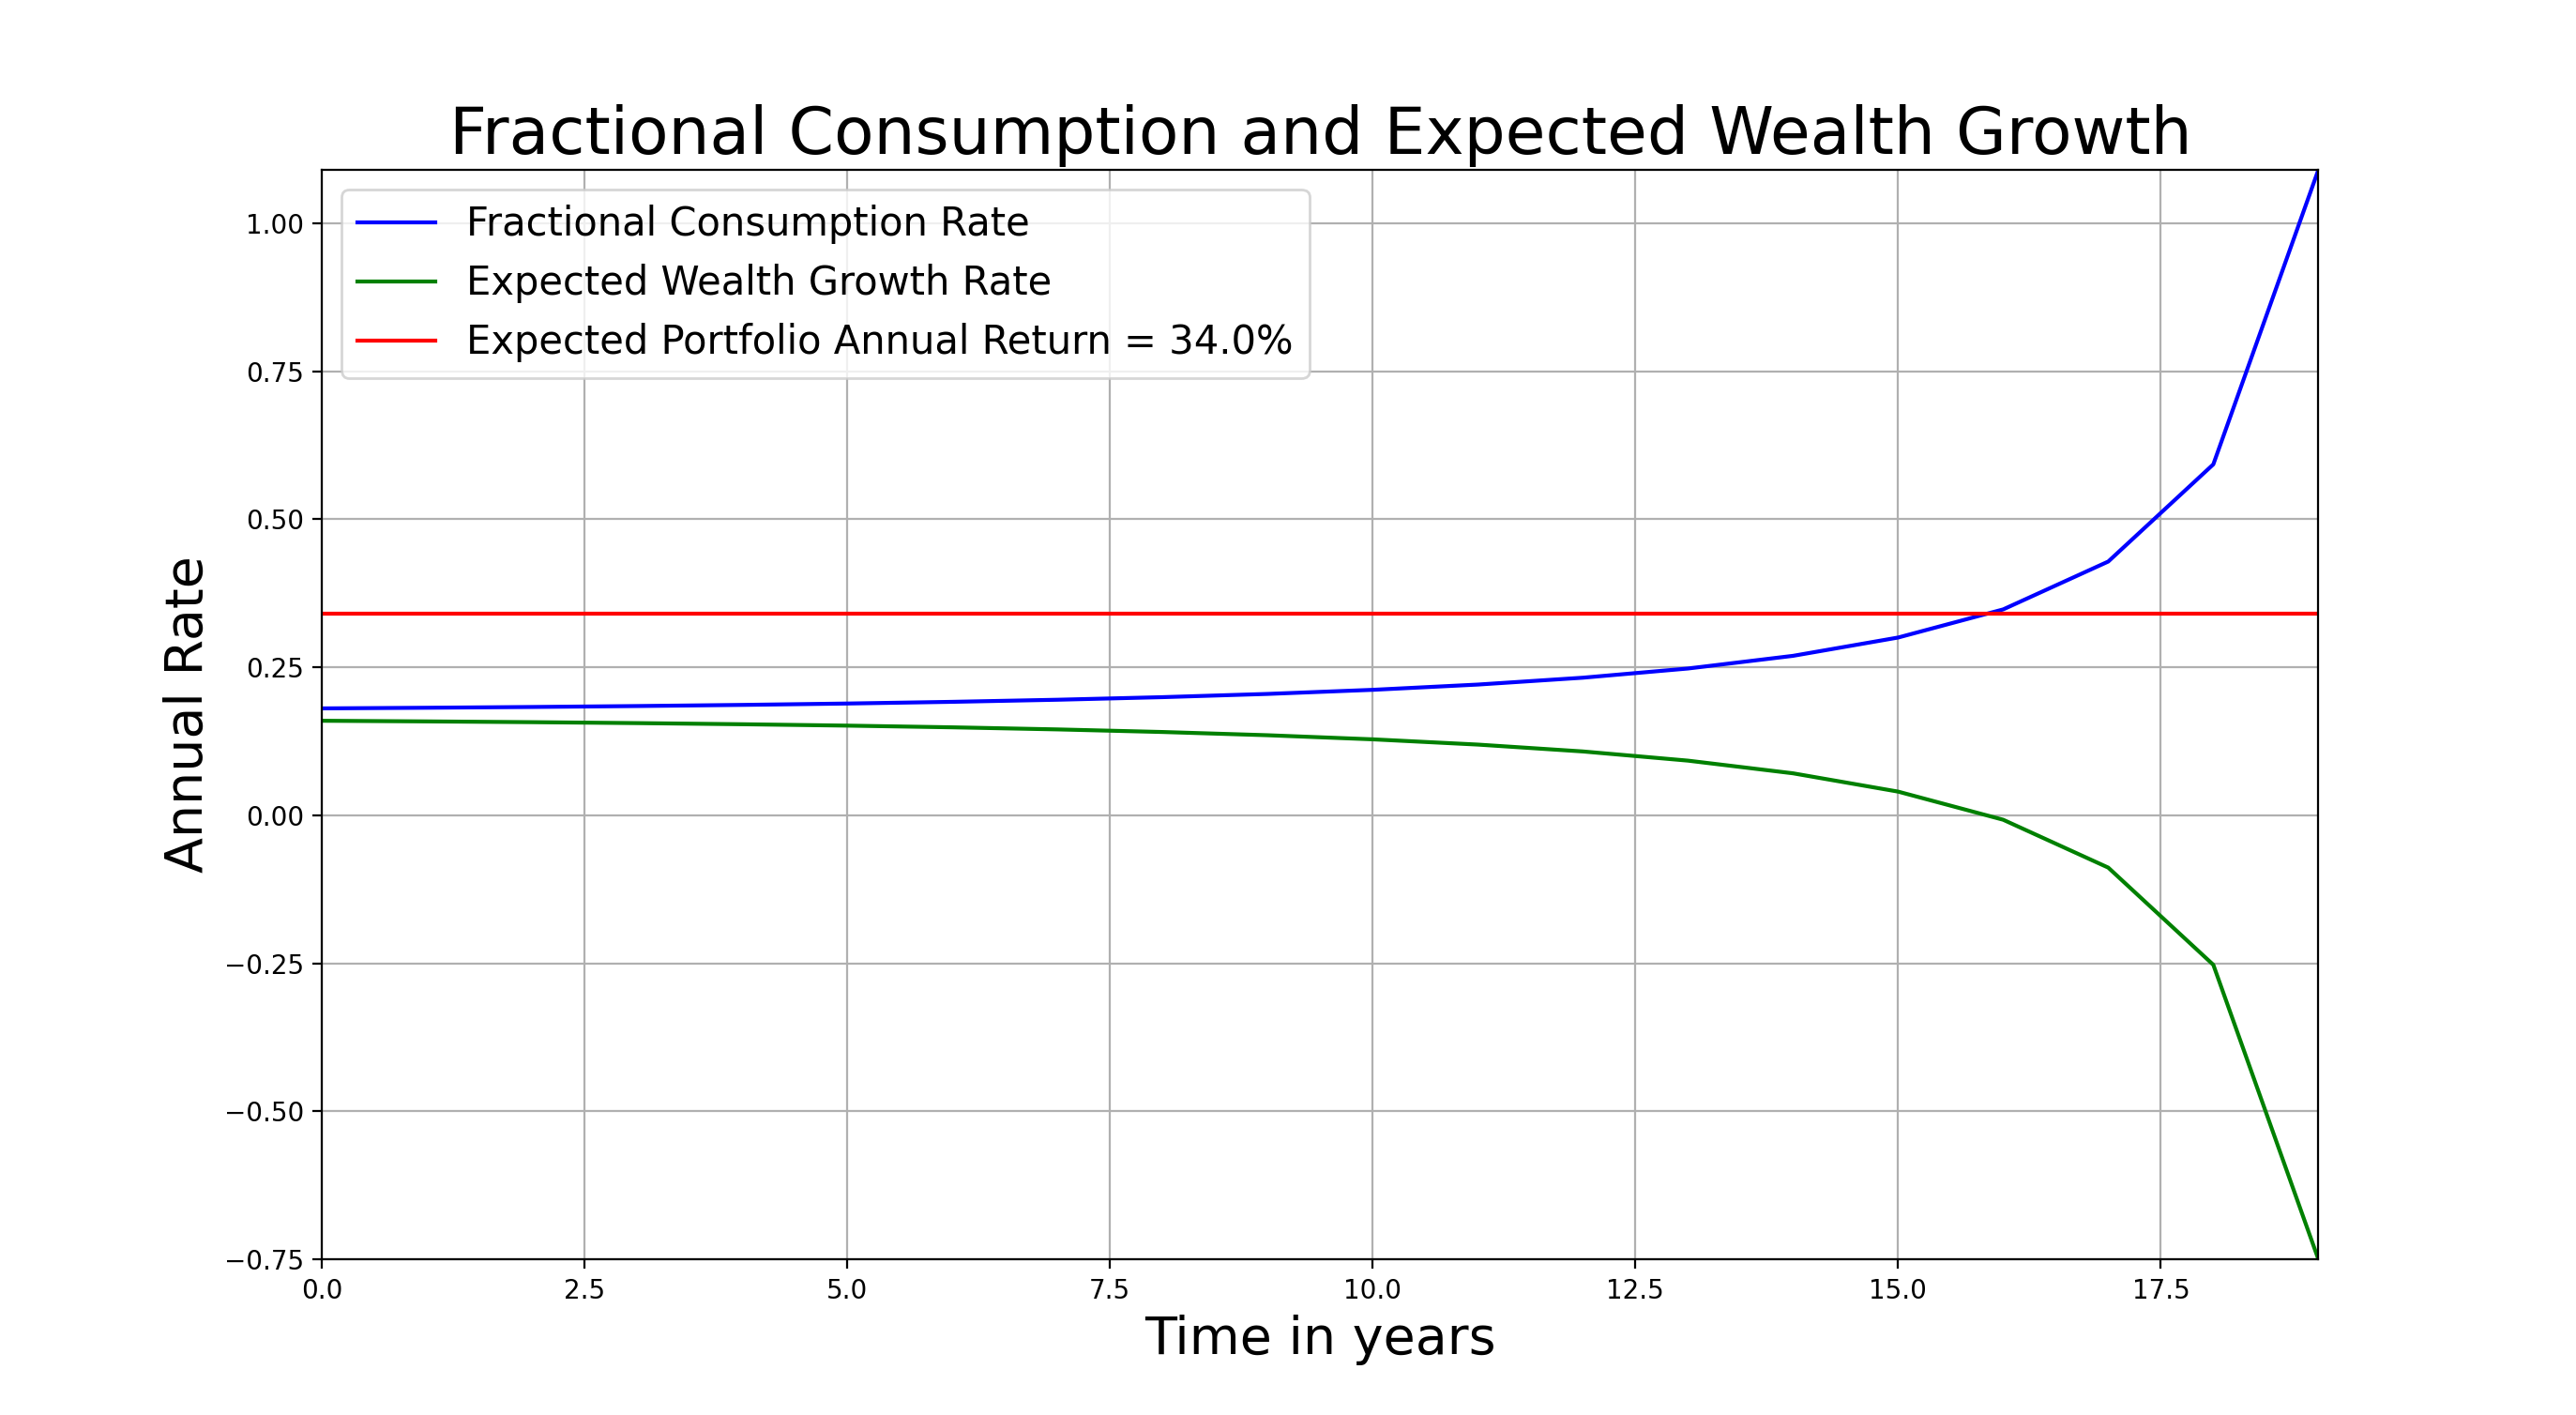
\includegraphics[width=12cm, height=8cm]{../finance/cme241/portfolio_growth.png}
\end{frame}

\begin{frame}
\frametitle{P1: Time-Trajectory of Expected Wealth}
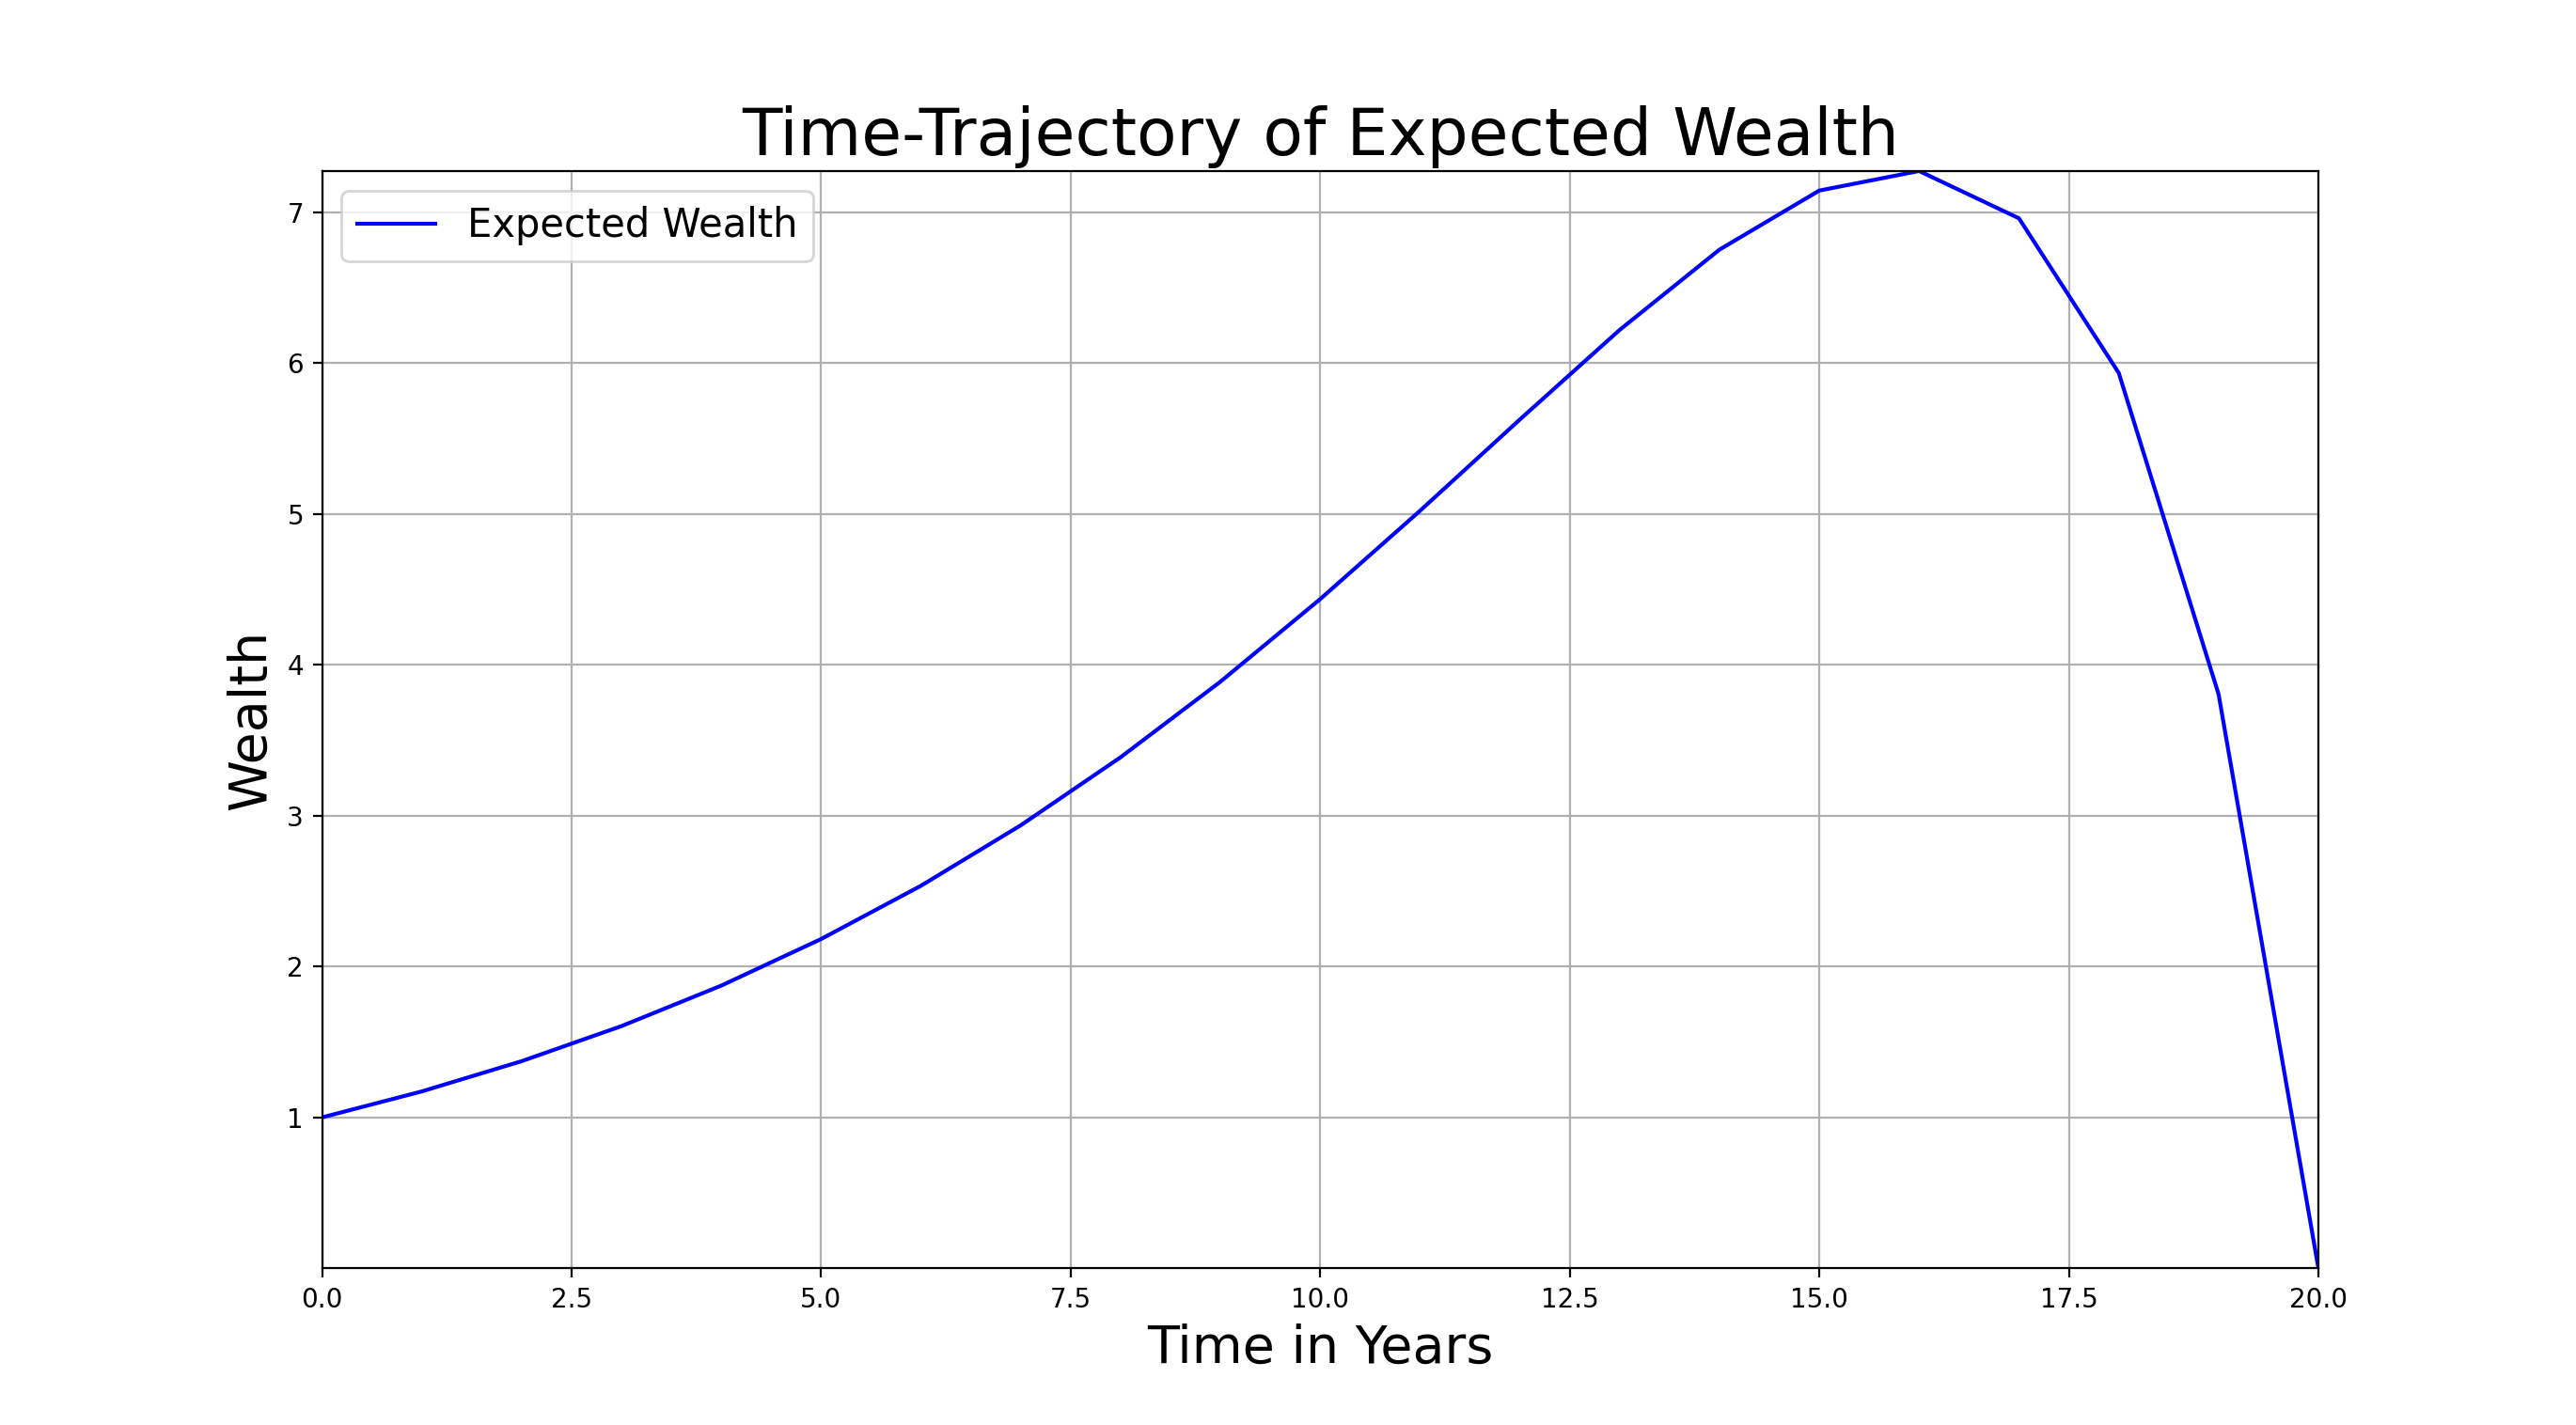
\includegraphics[width=12cm, height=8cm]{../finance/cme241/wealth_trajectory.png}
\end{frame}

\begin{frame}
\frametitle{P1: Real-World}
\pause
\begin{itemize}[<+->]
\item Analytical tractability in Merton's formulation is due to:
\begin{itemize}
\item Normal distribution of asset returns
\item Constant Relative Risk-Aversion
\item Frictionless, continuous trading
\end{itemize}
\item However, real-world situation involves:
\begin{itemize}
\item Discrete amounts of assets to hold and discrete quantities of trades
\item Transaction costs
\item Locked-out days for trading
\item Non-stationary/arbitrary/correlated processes of multiple assets
\item Changing/uncertain risk-free rate
\item Consumption constraints
\item Arbitrary Risk-Aversion/Utility specification
\end{itemize}
\item Practically we cannot hope to estimate a {\em Probabilities Model}
\item Build a practical simulator of market/constraints and do RL
\item Large Action Space points to Policy Gradient Algorithms
\end{itemize}
\end{frame}

\begin{frame}
\frametitle{P2: Classical Pricing and Hedging of Derivatives}
\pause
\begin{itemize}[<+->]
\item Classical Pricing/Hedging Theory is based on a few core concepts:
\begin{itemize}
\item {\bf Arbitrage-Free Market} - where you cannot make money from nothing
\item {\bf Replication} - when the payoff of a {\em Derivative} can be constructed by assembling (and rebalancing) a portfolio of the underlying securities
\item {\bf Complete Market} - where payoffs of all derivatives can be replicated
\item {\bf Risk-Neutral Measure} - Altered probability measure for movements of underlying securities for mathematical convenience in pricing
\end{itemize}

\item Assumptions of \href{https://github.com/coverdrive/technical-documents/blob/master/finance/ArbitrageCompleteness.pdf}{\underline{\textcolor{blue}{arbitrage-free and completeness}}}
lead to (dynamic, exact, unique) replication of derivatives with the underlying securities
\item Assumptions of frictionless trading provide these idealistic conditions
\item Frictionless := continuous trading, any volume, no transaction costs
\item Replication strategy gives us the pricing and hedging solutions
\item This is the foundation of the famous Black-Scholes formulas
\item However, the real-world has many frictions $\Rightarrow$ {\em Incomplete Market}
\item ... where derivatives cannot be exactly replicated
\end{itemize}
\end{frame}

\begin{frame}
\frametitle{P2: Pricing and Hedging in an Incomplete Market}
\pause
\begin{itemize}[<+->]
\item In an incomplete market, we have multiple risk-neutral measures
\item So, multiple derivative prices (each consistent with no-arbitrage)
\item The market/trader ``chooses'' a risk-neutral measure (hence, price)
\item This ``choice'' is typically made in ad-hoc and inconsistent ways
\item Alternative approach is for a trader to play {\em Portfolio Optimization}
\item Maximizing ``risk-adjusted return'' of the derivative plus hedges
\item Based on a specified preference for trading risk versus return
\item This preference is equivalent to specifying a \href{https://github.com/coverdrive/technical-documents/blob/master/finance/cme241/UtilityTheoryForRisk.pdf}{\underline{\textcolor{blue}{Utility function}}}
\item Reminiscent of the Portfolio Optimization problem we've seen before
\item Likewise, we can set this up as a stochastic control (MDP) problem
\item Where the decision at each time step is: {\em Trades in the hedges}
\item So what's the best way to solve this MDP?
\end{itemize}
\end{frame}


\begin{frame}
\frametitle{P2: Deep Reinforcement Learning (DRL)}
\pause
\begin{itemize}[<+->]
\item Dynamic Programming not suitable in practice due to:
\begin{itemize}
\item Curse of Dimensionality
\item Curse of Modeling
\end{itemize}
\item So we solve the MDP with {\em Deep Reinforcement Learning} (DRL)
\item The idea is to use real market data and real market frictions
\item Developing realistic simulations to derive the optimal policy
\item The optimal policy gives us the (practical) hedging strategy
\item The optimal value function gives us the price (valuation)
\item Formulation based on \href{https://papers.ssrn.com/sol3/papers.cfm?abstract_id=3355706}{\underline{\textcolor{blue}{Deep Hedging paper}}} by J.P.Morgan researchers
\item More details in the \href{https://papers.ssrn.com/sol3/papers.cfm?abstract_id=3355706}{\underline{\textcolor{blue}{prior paper}}} by some of the same authors
\end{itemize}
\end{frame}

\begin{frame}
\frametitle{P2: Problem Setup}
\pause
\begin{itemize}[<+->]
\item Let's simplify the problem setup a bit for ease of exposition
\item This model works for more complex, more frictionful markets too
\item Assume time is in discrete (finite) steps $t = 0, 1, \ldots, T$
\item Assume we have a position (portfolio) $D$ in $m$ derivatives
\item Assume each of these $m$ derivatives expires in time $ \leq T$
\item Portfolio-aggregated {\em Contingent Cashflows} at time $t$ denoted $X_t \in \mathbb{R}$
\item Assume we have $n$ underlying market securities as potential hedges
\item Hedge positions (units held) at time $t$ denoted $\bm{\alpha}_t \in \mathbb{R}^n$
\item Cashflows per unit of hedges held at time $t$ denoted $\bm{Y}_t \in \mathbb{R}^n$
\item Prices per unit of hedges at time $t$ denoted $\bm{P}_t \in \mathbb{R}^n$
\item PnL position at time $t$ is denoted as $\beta_t \in \mathbb{R}$
\end{itemize}
\end{frame}

\begin{frame}
\frametitle{P2: States and Actions}
\pause
\begin{itemize}[<+->]
\item Among other things, {\em State} $s_t \in \mathcal{S}_t$ contains $\bm{\alpha}_t, \bm{P}_t, \beta_t, D$
\item $s_t$ will include any market information relevant to trading actions
\item For simplicity, we assume $s_t$ is just the tuple $(\bm{\alpha}_t, \bm{P}_t, \beta_t, D)$
\item Denote {\em Action} at time $t$ as $\bm{a}_t \in \mathcal{A}_t$
\item $a_t$ represents units of hedges traded (positive for buy, negative for sell)
\item Trading restrictions (eg: no short-selling) define $\mathcal{A}_t$ as a function of $s_t$
\item State transitions $\bm{P}_{t+1}|\bm{P}_t$ available from a {\em simulator}, whose internals are estimated from real market data and realistic assumptions
\end{itemize}
\end{frame}

\begin{frame}
\frametitle{P2: Sequence of events at each time step $t=0, \ldots, T$}
\pause
\begin{enumerate}[<+->]
\item Observe state $s_t = (\bm{\alpha}_t, \bm{P}_t, \beta_t, D)$
\item Perform action (trades) $a_t$ to produce trading PnL $= - \bm{a}_t^T \cdot \bm{P}_t$
\item Trading transaction costs, eg. $= - \gamma \cdot abs(\bm{a}_t^T) \cdot \bm{P}_t$ for some $\gamma > 0$
\item Update $\bm{\alpha}_t$ as: $\bm{\alpha}_{t+1} = \bm{\alpha}_t + \bm{a}_t$ (force-liquidation at $T \Rightarrow \bm{a}_T= -\bm{\alpha}_T$)
\item Realize cashflows (from updated positions) $=X_{t+1} + \bm{\alpha}_{t+1}^T \cdot \bm{Y}_{t+1}$
\item Update PnL $\beta_t$ as:
$$\beta_{t+1} = \beta_t - \bm{a}_t^T \cdot \bm{P}_t - \gamma \cdot abs(\bm{a}_t^T) \cdot \bm{P}_t + X_{t+1} + \bm{\alpha}_{t+1}^T \cdot \bm{Y}_{t+1}$$
\item Reward $r_t = 0$ for all $t = 0, \ldots, T-1$ and $r_T = U(\beta_{T+1})$ for an appropriate concave Utility function $U$ (based on risk-aversion)
\item Simulator evolves hedge prices from $\bm{P}_t$ to $\bm{P}_{t+1}$
\end{enumerate}
\end{frame}

\begin{frame}
\frametitle{P2: Pricing and Hedging}
\pause
\begin{itemize}[<+->]
\item Assume we now want to enter into an incremental position (portfolio) $D'$ in $m'$ derivatives (denote the combined position as $D \cup D'$)
\item We want to determine the {\em Price} of the incremental position $D'$, as well as the hedging strategy for $D'$
\item Denote the Optimal Value Function at time $t$ as $V_t^* : \mathcal{S}_t \rightarrow \mathbb{R}$
\item Pricing of $D'$ is based on the principle that introducing the incremental position of $D'$ together with a calibrated cashflow (Price) at $t=0$ should leave the Optimal Value (at $t=0$) unchanged
\item Precisely, Price of $D'$ is the value $x$ such that
$$V_0^*((\bm{\alpha}_0, \bm{P}_0, \beta_0 - x, D \cup D')) = V_0^*((\bm{\alpha}_0, \bm{P}_0, \beta_0, D))$$
\item This Pricing principle is known as the principle of {\em Indifference Pricing}
\item The hedging strategy at time $t$ for all $0 \leq t < T$ is given by the Optimal Policy $\pi_t^* : \mathcal{S}_t \rightarrow \mathcal{A}_t$
\end{itemize}
\end{frame}

\begin{frame}
\frametitle{P2: DRL Approach relevant for Practical Trading?}
\pause
\begin{itemize}[<+->]
\item The industry practice/tradition has been to start with {\em Complete Market} assumption, and then layer ad-hoc/unsatisfactory adjustments
\item There is some past work on pricing/hedging in incomplete markets
\item But it's theoretical and not usable in real trading (eg: Superhedging)
\item This DRL approach should be explored more for practical trading
\item Key advantages of this DRL approach:
\begin{itemize}
\item Algorithm for pricing/hedging independent of market dynamics
\item Computational cost scales efficiently with size $m$ of derivatives portfolio
\item Enables one to faithfully capture practical trading situations/constraints
\item Deep Neural Networks provide great function approximation for RL 
\end{itemize}
\end{itemize}
\end{frame}

\begin{frame}
\frametitle{P3: Stopping Time}
\pause
\begin{itemize}[<+->]
\item Stopping time $\tau$ is a ``random time'' (random variable) interpreted as time at which a given stochastic process exhibits certain behavior
\item Stopping time often defined by a ``stopping policy'' to decide whether to continue/stop a process based on present position and past events
\item Deciding whether $\tau \leq t$ only depends on information up to time $t$
\item Hitting time of a Borel set $A$ for a process $X_t$ is the first time $X_t$ takes a value within the set $A$
\item Hitting time is an example of stopping time. Formally, 
$$T_{X,A} = \min \{t \in \mathbb{R} | X_t \in A\}$$
eg: Hitting time of a process to exceed a certain fixed level
\end{itemize}
\end{frame}

\begin{frame}
\frametitle{P3: Optimal Stopping Problem}
\pause
\begin{itemize}[<+->]
\item Optimal Stopping problem for Stochastic Process $X_t$: 
$$W(x) = \max_{\tau} \mathbb{E}[H(X_{\tau})|X_0 = x]$$
 where $\tau$ is a set of stopping times of $X_t$, $W(\cdot)$ is called the Value function, and $H$ is the Reward function.
\item Note that sometimes we can have several stopping times that maximize $\mathbb{E}[H(X_{\tau})]$ and we say that the optimal stopping time
is the smallest stopping time achieving the maximum value.
\item Example of Optimal Stopping: Optimal Exercise of American Options
\begin{itemize}
\item $X_t$ is risk-neutral process for underlying security's price
\item $x$ is underlying security's current price
\item $\tau$ is set of exercise times corresponding to various stopping policies
\item $W(\cdot)$ is American option price as function of underlying's current price
\item $H(\cdot)$ is the option payoff function, adjusted for time-discounting
\end{itemize}
\end{itemize}
\end{frame}


\begin{frame}
\frametitle{P3: Optimal Stopping Problems as MDPs}
\pause
\begin{itemize}[<+->]
\item We formulate Stopping Time problems as Markov Decision Processes
\item {\em State} is $X_t$
\item {\em Action} is Boolean: Stop or Continue
\item {\em Reward} always 0, except upon Stopping (when it is $=H(X_{\tau})$)
\item {\em State}-transitions governed by the Stochastic Process $X_t$
\item For discrete time steps, the Bellman Optimality Equation is:
$$V^*(X_t) = \max(H(X_t), \mathbb{E}[V^*(X_{t+1})|X_t])$$
\item For finite number of time steps, we can do a simple backward induction algorithm from final time step back to time step 0
\end{itemize}
\end{frame}


\begin{frame}
\frametitle{P3: Mainstream approaches to American Option Pricing}
\pause
\begin{itemize}[<+->]
\item American Option Pricing is Optimal Stopping, and hence an MDP
\item So can be tackled with Dynamic Programming or RL algorithms
\item But let us first review the mainstream approaches
\item For some American options, just price the European, eg: vanilla call
\item When payoff is not path-dependent and state dimension is not large, we can do backward induction on a binomial/trinomial tree/grid
\item Otherwise, the standard approach is \href{https://people.math.ethz.ch/~hjfurrer/teaching/LongstaffSchwartzAmericanOptionsLeastSquareMonteCarlo.pdf}{\underline{\textcolor{blue}{Longstaff-Schwartz algorithm}}}
\item Longstaff-Schwartz algorithm combines 3 ideas:
\begin{itemize}
\item Valuation based on Monte-Carlo simulation
\item Function approximation of continuation value for in-the-money states
\item Backward-recursive determination of early exercise states
\end{itemize}
\item RL is an attractive alternative to Longstaff-Schwartz algorithm
\item LSPI and Deep Q-Learning solutions sketched \href{https://github.com/coverdrive/technical-documents/blob/master/finance/cme241/Tour-Batch.pdf}{\underline{\textcolor{blue}{here}}}
\end{itemize}
\end{frame}

\begin{frame}
\frametitle{P4: Trading Order Book (abbrev. OB)}
\includegraphics[width=11.5cm, height=7cm]{../finance/cme241/order_book.png}
\end{frame}

\begin{frame}
\frametitle{P4: Basics of Order Book (OB)}
\pause
\begin{itemize}[<+->]
\item Buyers/Sellers express their intent to trade by submitting bids/asks
\item These are Limit Orders (LO) with a price $P$ and size $N$
\item Buy LO $(P, N)$ states willingness to buy $N$ shares at a price $\leq P$
\item Sell  LO $(P, N)$ states willingness to sell $N$ shares at a price $\geq P$
\item Order Book aggregates order sizes for each unique price
\item So we can represent with two sorted lists of (Price, Size) pairs
$$\mbox{Bids: } [(P_i^{(b)}, N_i^{(b)}) \mid 0 \leq i < m], P_i^{(b)} > P_j^{(b)} \mbox{ for } i < j$$
$$\mbox{Asks: } [(P_i^{(a)}, N_i^{(a)}) \mid 0 \leq i < n], P_i^{(a)} < P_j^{(a)} \mbox{ for } i < j$$
\item We call $P_0^{(b)}$ as simply {\em Bid}, $P_0^{(a)}$ as {\em Ask}, $\frac {P_0^{(a)} + P_0^{(b)}} 2$ as {\em Mid}
\item We call $P_0^{(a)} - P_0^{(b)}$ as {\em Spread}, $P_{n-1}^{(a)} - P_{m-1}^{(b)}$ as {\em Market Depth}
\item A Market Order (MO) states intent to buy/sell $N$ shares at the {\em best possible price(s)} available on the OB at the time of MO submission
\end{itemize}
\end{frame}

\begin{frame}
\frametitle{P4: Order Book (OB) Activity}
\pause
\begin{itemize}[<+->]
\item A new Sell LO $(P,N)$ potentially removes best bid prices on the OB
$$\mbox{Removal: } [(P_i^{(b)}, \min(N_i^{(b)}, \max(0, N - \sum_{j=0}^{i-1} N_j^{(b)}))) \mid (i: P_i^{(b)} \geq P)]$$
\item After this removal, it adds the following to the asks side of the OB 
$$(P, \max(0, N - \sum_{i: P_i^{(b)} \geq P}  N_i^{(b)}))$$
\item A new Buy LO operates analogously (on the other side of the OB)
\item A Sell Market Order $N$ will remove the best bid prices on the OB
$$\mbox{Removal: } [(P_i^{(b)}, \min(N_i^{(b)}, \max(0, N - \sum_{j=0}^{i-1} N_j^{(b)}))) \mid 0 \leq i < m]$$
\item A Buy Market Order $N$ will remove the best ask prices on the OB
$$\mbox{Removal: } [(P_i^{(a)}, \min(N_i^{(a)}, \max(0, N - \sum_{j=0}^{i-1} N_j^{(a)}))) \mid 0 \leq i < n]$$
\end{itemize}
\end{frame}

\begin{frame}
\frametitle{P4: Price Impact and Order Book Dynamics}
\pause
\begin{itemize}[<+->]
\item We focus on how a Market order (MO) alters the OB
\item A large-sized MO often results in a big {\em Spread} which could soon be replenished by new LOs, potentially from either side
\item So a large-sized MO moves the Bid/Ask/Mid ({\em Price Impact} of MO)
\item Subsequent Replenishment activity is part of {\em OB Dynamics}
\item Models for OB Dynamics can be quite complex
\end{itemize}
\end{frame}

\begin{frame}
\frametitle{P4: Optimal Trade Order Execution Problem}
\pause
\begin{itemize}[<+->]
\item The task is to sell a large number $N$ of shares
\item We are allowed to trade in $T$ discrete time steps
\item We are only allowed to submit Market Orders
\item Need to consider both {\em Temporary} and {\em Permanent} Price Impact
\item For simplicity, consider a model of just the {\em Bid Price} Dynamics
\item Goal is to maximize Expected Total Utility of Sales Proceeds
\item By breaking $N$ into appropriate chunks (timed appropriately)
\item If we sell too fast, we are likely to get poor prices
\item If we sell too slow, we risk running out of time
\item Selling slowly also leads to more uncertain proceeds (lower Utility)
\item This is a Dynamic Optimization problem
\item We can model this problem as a Markov Decision Process (MDP)
\end{itemize}
\end{frame}

\begin{frame}
\frametitle{P4: Problem Notation}
\pause
\begin{itemize}[<+->]
\item Time steps indexed by $t = 0, 1, \ldots, T$
\item $P_t$ denotes Bid Price at start of time step $t$
\item $N_t$ denotes number of shares sold in time step $t$
\item $R_t = N - \sum_{i=0}^{t-1}N_i = $ shares remaining to be sold at start of step $t$
\item $R_0 = N, R_{t+1}  = R_t - N_t \text{ for all } t < T, N_{T-1} = R_{T-1} \Rightarrow R_T = 0$
\item Price Dynamics given by:
$$P_{t+1} = f_t(P_t, N_t, \epsilon_t)$$
where $f_t(\cdot)$ is an arbitrary function incorporating:
\begin{itemize}
\item Permanent Price Impact of selling $N_t$ shares
\item Impact-independent market-movement of Bid Price over time step $t$
\item $\epsilon_t$ denotes source of randomness in Bid Price market-movement
\end{itemize}
\item Sales Proceeds in time step $t$ defined as:
$$N_t \cdot Q_t = N_t \cdot (P_t - g_t(P_t, N_t))$$
where $g_t(\cdot)$ is an arbitrary func representing Temporary Price Impact
\item Utility of Sales Proceeds function denoted as $U(\cdot)$
\end{itemize}
\end{frame}

\begin{frame}
\frametitle{P4: Markov Decision Process (MDP) Formulation}
\pause
\begin{itemize}[<+->]
\item This is a discrete-time, finite-horizon MDP
\item MDP Horizon is time $T$, meaning all states at time $T$ are terminal
\item Order of MDP activity in each time step $0 \leq t < T$:
\begin{itemize}
\item Observe {\em State} $s_t := (P_t, R_t) \in \mathcal{S}_t$
\item Perform {\em Action} $a_t := N_t \in \mathcal{A}_t$
\item Receive {\em Reward} $r_{t+1} := U(N_t \cdot Q_t) = U(N_t \cdot (P_t - g_t(P_t, N_t)))$
\item Experience Price Dynamics $P_{t+1} = f_t(P_t, N_t, \epsilon_t)$
\end{itemize}
\item Goal is to find a Policy $\pi^*_t((P_t, R_t)) = N_t^*$ that maximizes: $$\mathbb{E}[\sum_{t=0}^{T-1} \gamma^t \cdot U(N_t \cdot Q_t)] \mbox{ where } \gamma \mbox{ is MDP discount factor}$$
\item \href{http://alo.mit.edu/wp-content/uploads/2015/06/Optimal-Control-of-Execution-Costs.pdf}{\underline{\textcolor{blue}{Closed-form solutions by Bertsimas-Lo}}}
\item \href{https://www.math.nyu.edu/faculty/chriss/optliq_f.pdf}{\underline{\textcolor{blue}{Risk-Aversion considerations by Almgren-Chriss}}}
\end{itemize}
\end{frame}

\begin{frame}
\frametitle{P4: Real-world Optimal Trade Order Execution}
\pause
\begin{itemize}[<+->]
\item Arbitrary Price Dynamics $f_t(\cdot)$ and Temporary Price Impact $g_t(\cdot)$
\item Non-stationarity/non-linear dynamics/impact require (Numerical) DP
\item Frictions: Discrete Prices/Sizes, Constraints on Prices/Sizes, Fees
\item Incorporating various markets factors in the State bloats State Space
\item We could also represent the entire OB within the State
\item Practical route is to develop a simulator capturing all of the above
\item Simulator is a {\em Market-Data-learnt Sampling Model} of OB Dynamics 
\item In practice, we'd need to also capture {\em Cross-Asset Market Impact}
\item Using this simulator and neural-networks func approx, we can do RL
\item References: \href{https://www.cis.upenn.edu/~mkearns/papers/rlexec.pdf}{\underline{\textcolor{blue}{Nevmyvaka, Feng, Kearns; 2006}}} and \href{https://arxiv.org/pdf/1906.02312.pdf}{\underline{\textcolor{blue}{Vyetrenko, Xu; 2019}}}
\item Exciting area for Future Research as well as Engineering Design
\end{itemize}
\end{frame}

\begin{frame}
\frametitle{P5: OB Dynamics and Market-Making}
\pause
\begin{itemize}[<+->]
\item Modeling OB Dynamics involves predicting arrival of MOs and LOs
\item Market-makers are liquidity providers (providers of Buy and Sell LOs)
\item Other market participants are typically liquidity takers (MOs)
\item But there are also other market participants that trade with LOs
\item Complex interplay between market-makers \& other mkt participants
\item Hence, OB Dynamics tend to be quite complex
\item We view the OB from the perspective of a single market-maker who aims to gain with Buy/Sell LOs of appropriate width/size
\item By anticipating OB Dynamics \& dynamically adjusting Buy/Sell LOs
\item Goal is to maximize {\em Utility of Gains} at the end of a suitable horizon
\item If Buy/Sell LOs are too narrow, more frequent but small gains
\item If Buy/Sell LOs are too wide, less frequent but large gains
\item Market-maker also needs to manage potential unfavorable inventory (long or short) buildup and consequent unfavorable liquidation
\end{itemize}
\end{frame}



\begin{frame}
\frametitle{P5: Notation for Optimal Market-Making Problem}
\pause
\begin{itemize}[<+->]
\item We simplify the setting for ease of exposition
\item Assume finite time steps indexed by $t= 0, 1, \ldots, T$
\item Denote $W_t \in \mathbb{R}$ as Market-maker's trading PnL at time $t$
\item Denote $I_t \in \mathbb{Z}$ as Market-maker's inventory of shares at $t$ ($I_0 = 0$)
\item $S_t \in \mathbb{R}^+$ is the OB Mid Price at time $t$ (assume stochastic process)
\item $P_t^{(b)} \in \mathbb{R}^+, N_t^{(b)} \in \mathbb{Z}^+$ are market maker's Bid Price, Bid Size at $t$
\item $P_t^{(a)} \in \mathbb{R}^+, N_t^{(a)} \in \mathbb{Z}^+$ are market-maker's Ask Price, Ask Size at $t$
\item Assume market-maker can add or remove bids/asks costlessly
\item Random var $X_t^{(b)} \in \mathbb{Z}_{\geq 0}$ denotes bid-shares ``hit'' {\em up to} time $t$
\item Random var $X_t^{(a)} \in \mathbb{Z}_{\geq 0}$ denotes ask-shares ``lifted'' {\em up to} time $t$
$$W_{t+1} = W_t + P_t^{(a)} \cdot (X_{t+1}^{(a)} - X_t^{(a)}) - P_t^{(b)} \cdot (X_{t+1}^{(b)} - X_t^{(b)}) \mbox{ , } I_t = X_t^{(b)} - X_t^{(a)}$$
\item Goal to maximize $\mathbb{E}[U(W_T + I_T \cdot S_T)]$ for appropriate concave $U(\cdot)$
\end{itemize}
\end{frame}

\begin{frame}
\frametitle{P5: Markov Decision Process (MDP) Formulation}
\pause
\begin{itemize}[<+->]
\item Order of MDP activity in each time step $0 \leq t \leq T-1$:
\begin{itemize}
\item Observe {\em State} $:= (S_t, W_t, I_t) \in \mathcal{S}_t$
\item Perform {\em Action} $:= (P_t^{(b)}, N_t^{(b)}, P_t^{(a)}, N_t^{(a)}) \in \mathcal{A}_t$
\item Experience OB Dynamics resulting in:
\begin{itemize}
\item random bid-shares hit $=X_{t+1}^{(b)} - X_t^{(b)}$ and ask-shares lifted $=X_{t+1}^{(a)} - X_t^{(a)}$
\item update of $W_t$ to $W_{t+1}$, update of $I_t$ to $I_{t+1}$
\item stochastic evolution of $S_t$ to $S_{t+1}$
\end{itemize}
\item Receive next-step ($t+1$) {\em Reward} $R_{t+1}$
$$
R_{t+1} :=
\begin{cases}
0 & \text{ for }1 \leq t+1 \leq T-1 \\
U(W_{t+1} + I_{t+1} \cdot S_{t+1}) & \text{ for } t+1 = T \\
\end{cases}
$$
\end{itemize}
\item Goal is to find an {\em Optimal Policy} $\pi^* = (\pi_0^*, \pi_1^*, \ldots, \pi_{T-1}^*)$:
$$\pi_t^*((S_t, W_t, I_t)) = (P_t^{(b)}, N_t^{(b)}, P_t^{(a)}, N_t^{(a)}) \mbox{ that maximizes } \mathbb{E}[R_T]$$
\end{itemize}
\end{frame}


\begin{frame}
\frametitle{P5: Real-world Market-Making and RL}
\pause
\begin{itemize}[<+->]
\item \href{https://www.math.nyu.edu/faculty/avellane/HighFrequencyTrading.pdf}{\underline{\textcolor{blue}{Avellaneda and Stoikov}}} derive a closed-form solution for a simple continuous-time formulation
\item Real-world OB dynamics are non-stationary, non-linear, complex
\item Frictions: Discrete Prices/Sizes, Constraints on Prices/Sizes, Fees
\item Need to capture various market factors in the {\em State} \& OB Dynamics
\item This leads to Curse of Dimensionality and Curse of Modeling
\item The practical route is to develop a simulator capturing all of the above
\item Simulator is a {\em Market-Data-learnt Sampling Model} of OB Dynamics 
\item Using this simulator and neural-networks func approx, we can do RL
\item References: \href{https://arxiv.org/pdf/1804.04216.pdf}{\underline{\textcolor{blue}{2018 Paper from University of Liverpool}}} and 
\href{https://arxiv.org/pdf/1911.05892.pdf}{\underline{\textcolor{blue}{2019 Paper from JP Morgan Research}}}
\item Exciting area for Future Research as well as Engineering Design
\end{itemize}
\end{frame}

\end{document}